\documentstyle[titlepage]{article}

\parindent = 0cm
\parskip = 0.1cm

\newcommand{\ie}{{\em i.e.\/}}
\newcommand{\eg}{{\em e.g.\/}}
\newcommand{\etc}{{\em etc.\/}}

\input{psfig}

\begin{document}

\begin{titlepage}
\begin{center}
\vspace{7cm}
{\Huge Programmer's \\ Reference Manual \\ to \\ the Kinetic Compiler \\
  version 1.00} \\
\vspace{2cm}
{\Large Kenneth Geisshirt \\ 
{\normalsize kneth@osc.kiku.dk} \\
Department of Theoretical Chemistry \\
H.C. {\O}rsted Institute \\
Universitetsparken 5 \\
2100 K{\o}benhavn {\O} \\
Denmark } \\
\vspace{3cm}
{\Large 9 October 1994}
\end{center}
\end{titlepage}

\bibliographystyle{plain}
\tableofcontents
\newpage

\section{Introduction}
This manual is the technical documentation of {\tt kc}. The version 
described is 1.00. The paper contains information on the data types 
used in the program \ie the interface is given in all details. The group
of readers is thought as future programmers, who is going to extend
and maintain the program. 

The grammar wil also be explained. The parser and the 
lexical analyser will briefly discussed as well.

The reader is assumed to have knowledge of (ANSI) C, \cite{KR}, 
LALR-grammars, \cite{ctools}, \cite{dragon}, \cite{LexYacc}, 
concrete data types, \cite{decker} and Unix in general.
There exists also a user's manual to the system, \cite{kc-man}, and
the reader of this manual is recommended to this it before proceeding.

The manual is structured in the following way: Each section documents a
concrete data type, the parser or just a module. Each 
section begins with a small presentation and then the operations
follow, each in a distict subsection. All modules may be included
more than once, \ie just like the ordinary standard libraries.

The source files discussed in the manual are in general found in the
{\tt src} directory of the {\tt kc} tree.

\section{A brief overview}
The kinetic compiler is a compiler in the traditional understanding,
\ie it translate a given source language into a target language. The
source language is chemical reaction and ordinary differential
equations and the target language is subroutines for a simulation
program.

The general structure of {\tt kc} is found below. The figure shows the
data stream.

\begin{figure}
  \fbox{\psfig{file=stream.ps,width=13cm,height=8cm}}
  \caption{The data stream in the kinetic compiler.}
\end{figure}

The lexical analyser and the parser read the input file, and they
insert the information contained in the file into various tables, here
called the symbol table.

A natural data type of the system is general expressions. Especially
the code generators use expressions as well as the information stored
by the parser. The code generators is generating the output files.

The figure below shows a simplified dependency graph of the main
libraries of the program. Each library is shown as a box. The library
called ``Code generators'' should be understood as a typical code
generator.

\begin{figure}
  \fbox{\psfig{file=lib-dep.ps,width=13cm,height=8cm}}
  \caption{The dependency graph for the libraries.}
\end{figure}

\section{Data type TableMan}
\label{tableman}
The data type TableMan is found the the file {\tt tableman.h}. The
purpose of the data type is to keep track
of the information, which is read from the input file. The table
manager is actual seven tables in one - 
symbol table, reaction table, constraint table, dynamical variable
table, expression table\footnote{The tables of dynamical variables and
  expression are closely related.}, print table, 
and parameter table - but this does the programmer not be aware of.

\subsection{The {\tt Direc} type}
\label{direc}
This type is used in some of the operations, either as input or
output. The type is an enumerated type, and has three values. 

\vspace{0.2cm}
\begin{center}
\begin{tabular}{ll}
\hline
 Value  & Description      \\ \hline 
 uni    & one-way reaction \\ 
 bi     & two-ways reaction \\ 
 equi   & equilibrium       \\ 
\hline
\end{tabular}
\end{center}
\vspace{.2cm}

These three names and the type can be used, when the table manager is included.

\subsection{SetupTableMan}
\begin{verbatim}
void SetupTableMan(void)
\end{verbatim}
This procedure is setting up the table manager. It is to be called
before any other routine in the table manager and only once.

This routine will always return NoError.

\subsection{GetError}
\begin{verbatim}
TableErrors GetError(void)
\end{verbatim}
The function returns an error code from last used operation in the 
table manager. There are the following possible errors:

\vspace{.2cm}
\begin{center}
\begin{tabular}{ll}
\hline
Error name      & Description              \\ \hline 
NoError         & no error                 \\ 
TooManyConst    & constant table full      \\ 
TooManySpec     & species table full        \\ 
SpecAlready     & species already defined   \\ 
KonstAlready    & constant already defined \\ 
NonSpec         &                          \\ 
TooManyReact    & reaction table full      \\ 
WrongDirect     &                          \\ 
ReactAlready    & reaction already defined \\ 
NotFound        & a search was unsuccesful \\ 
TooManyConstrain & constraint table full   \\ 
TooManyDynVar   & dynamical table full     \\ 
TooManyExpr     & expression table full    \\ 
ExpreAlready    & expression already defined \\ 
TooManyPrn      & print table full         \\
TooManyParam    & parameter table full     \\
ParamAlready    & parameter aldreay defined \\
\hline
\end{tabular}
\end{center}
\vspace{.2cm}

The definition of these names are found in the type {\tt TableErrors},
which can be used when the table manager is included.

\subsection{NewSpecie}
\begin{verbatim}
void NewSpecie(char *name, double charge)
\end{verbatim}

The procedure defines a new species which has the name {\tt name} 
and the charge {\tt charge}. Radicals have the
charge {\tt MAXFLOAT} which is defined in standard header file {\tt values.h}. 

The possible errors are NoError, TooManySpec and SpecAlready. The last
will occur, if the species already has been defined. This may mean 
nothing and can be ignored. The second error is more problematic; I
do not have any solutions for that.

\subsection{NewConstant}
\begin{verbatim}
void NewConstant(char *name, double value)
\end{verbatim}

This procedure defines a new constant in the symbol table with name 
{\tt name} and the value {\tt value}. If
the constant already is defined the returned error is KonstAlready.

\subsection{NewDiffConst}
\begin{verbatim}
void NewDiffConst(char *name, double charge, double value)
\end{verbatim}

The procedure assigns new value to a diffusion constant. If the species {\tt 
name(charge)} has not been defined the error NonSpec is returned,
otherwise NoError.

This procedure should not be used - it is an old procedure. One should
use NewSpecConst instead, see section \ref{tableman:NewSpecConst}

\subsection{NewCoeff}
\label{newcoeff}
\begin{verbatim}
void NewCoeff(int react_no, char *name, double charge, 
              double coeff, int side)
\end{verbatim}

This routine assigns a new coefficient for the species {\tt
  name(charge)} in reaction number {\tt react\_no}. The routine is 
supporting autocatalytic reactions. 

If {\tt side} is 1 the the coefficient is inserted on the left side,
otherwise on the right hand side.

Please note, the procedure does {\em not} return any errors 
(not NoError neither).

\subsection{NewRateConst}
\begin{verbatim}
void NewRateConst(int react, int direc, Tree value)
\end{verbatim}

The procedure sets a new value ({\tt value}) for the rate constant 
in reaction {\tt react}. The parameter {\tt direc} gives the 
following possibilities.

\vspace{.2cm}
\begin{center}
\begin{tabular}{rl}
\hline
 Value      & Direction \\ \hline 
 -1         & $\rightarrow$ \\ 
 0          & = \\ 
 1          & $\leftarrow$ \\ 
\hline
\end{tabular}
\end{center}
\vspace{.2cm}

\subsection{NewBeginConc}
\begin{verbatim}
void NewBeginConc(char *name, double charge, double value)
\end{verbatim}

The NewBeginConc procedure sets a new initial concentration for species {\tt 
name(charge)}. The new value is the parameter {\tt value}. If the 
species is not defined, the error code is NonSpec.

\subsection{NewReaction}
\begin{verbatim}
void NewReaction(int react)
\end{verbatim}

This procedure prepares a new reaction with the number {\tt react}. 
There are three possible errors.
NoError will be the code, if the procedure was succesful. If there 
was no space (reaction table full) the error code is TooManyReact, while if the
reaction already has been defined, the error code is ReactAlready.

\subsection{AddReactionKind}
\begin{verbatim}
void AddReactionKind(int react, Direc direct)
\end{verbatim}

This procedure adds the direction to a given reaction. Details on the 
directions, see section \ref{direc}. The error code is not set in 
this operation, \ie it can be
dangerous to used it, if one is not absolutely sure on the reaction
number (commonly determined by GetCurrentReact).

\subsection{SpecieInReaction}
\begin{verbatim}
void SpecieInReaction(int react, char *name, double charge)
\end{verbatim}

This operation inserts a new species ({\tt name(charge)}) into the 
reaction table. The species is associated with reaction number 
{\tt react}. The coefficient that the species has in the reaction 
must be set by NewCoeff, see section \ref{newcoeff}. The reaction
number is during parsing determined by GetCurrentReact.

There is no setting of error codes in this operation.  

\subsection{NewConstraint}
\begin{verbatim}
void NewConstaint(char *name, double charge, Tree expr)
\end{verbatim}

This procedure prepares a new constraint. The error code is 
TooManyConstrain if there is no space in the table. All constraints
are assumed to be in the form

\begin{verbatim}
[J] = expr  
\end{verbatim}
where {\tt J} is the species, \ie {\tt name(charge)}.

\subsection{NumOfConstraint}
\begin{verbatim}
int NumOfConstraint(void)
\end{verbatim}

This function returns the number of constraints defined so far.

\subsection{GetConstraintNo}
\begin{verbatim}
void GetConstraintNo(int no, char *name, double *charge, Tree t)
\end{verbatim}

This function finds the constraint number {\tt no} in the constraint
table. The error code is NotFound if the constraint does not exist.
The species associated with the constraint is returned in the
parameters {\tt name} and {\tt charge}.

\subsection{GetReactNo}
\begin{verbatim}
int GetReactNo(int counter)
\end{verbatim}

This function returns the reaction number (as defined when it was 
created, \eg by the parser). The parameter {\tt counter} is the index
in the table of  
reactions. This function is {\em not} pretty when used, but can be useful.

\subsection{RenameSpec}
\begin{verbatim}
void RenameSpec(char *rename, char *name, double charge) 
\end{verbatim}

The operation renames the species {\tt name(charge)}, so both the name 
and the charge become part of the new name {\tt rename}. The parameter
{\tt rename} has to be allocated before the call, 
\eg by StringAlloc.

The new name will have the form {\tt name\_charge}, where the 
charge is converted so positive charge is $n$ times of {\tt p} and 
negative charge is $n$ times of {\tt n} ($n$ is the integer part
of the charge). If the charge shows that it is a radical, the 
suffix is {\tt rad}.

No error codes are returned.

\subsection{NoOfSpec}
\label{nospec}
\begin{verbatim}
int NoOfSpec(void)
\end{verbatim}

This function returns the number of species, which have been defined so far.

\subsection{GetFirstSpecA}
\label{GetA}
\begin{verbatim}
int GetFirstSpecA(int no, char *name, double *charge, 
                  double *coeff, int side)
\end{verbatim}

This function finds the first species in a in reaction {\tt no}. If no
species is found (or the reaction is not found) the function 
returns 0, otherwise 1. The found species is returned in the
parameters {\tt name} and {\tt charge}. The coefficient
is returned in parameter {\tt coeff}. The {\tt side} parameter has be
0 if the species is to be found on the left side, otherwise 1.

This function is meant to be used together with GetNextSpecA,
and GetFirstSpecA is the initial call.

\subsection{GetNextSpecA}
\begin{verbatim}
int GetNextSpecA(char *name, double *charge, double *coeff, 
                 int side)
\end{verbatim}

This function continues the search started by {\tt GetFirstSpecA}, 
see section \ref{GetA}. The returning values are also analogous to 
that function.

\subsection{GetCoeffInReact}
\begin{verbatim}
double GetCoeffInReact(int react_no, char *name, 
                       double charge, int side)
\end{verbatim}

The function returns the coefficient (if any) of the species
{\tt name(charge)} in reaction 
number {\tt react{\_}no}. The {\tt side} parameter determine the side of
the reaction to search; 0 is left side, 1 is the right side. The
function does not return any error codes.

\subsection{GetFirstSpecB}
\label{GetB}
\begin{verbatim}
int GetFirstSpecB(char *name, double *charge)
\end{verbatim}

The function finds the first species in the symbol table, if there 
is any. If the function
finds a species it returns 1, otherwise 0. The species is returned 
in the two parameters.

In a sense the routine (together with GetNextSpecB) is doing the same
as the NoOfSpec/GetSpecNo couple.

\subsection{GetNextSpecB}
\begin{verbatim}
int GetNextSpecB(char *name, double *charge)
\end{verbatim}

This function continues the search, which was begun by 
{\tt GetFirstSpecB}, see section \ref{GetB}.
The return values also analogue to that function.

\subsection{GetSpecNo}
\begin{verbatim}
void GetSpecNo(int count, char *name, double *charge)
\end{verbatim}

The procedure finds species number {\tt count} in the symbol table. 
The procedure returns the species in the two last parameters. 
If no species is found the return values are undefined.
It is only safe to let {\tt count} be between 1 and the number
returned by {\tt NoOfSpec}, see section \ref{nospec}.

\subsection{GetReactKind}
\begin{verbatim}
Direc GetReactKind(int react_no)
\end{verbatim}

This function returns the reaction kind as defined by the type 
{\tt Direc}, see section \ref{direc}.
The function has no error codes. The parameter {\tt react{\_}no} is the 
reaction number defined when the reaction was inserted into the table,
and not the index of the table.

\subsection{GetRateConst}
\begin{verbatim}
void GetRateConst(int react_no, Direc direct, int way, Tree value)
\end{verbatim}

The function returns the rate constant of the reaction {\tt
  react\_no}. 
The function has to known which kind of reaction it is (parameter 
{\tt direct}, see section \ref{direc}). 
For two-ways reactions the parameter selects which of the two
constants there is returned, i.e.
{\tt way} has only meaning when {\tt direct} = {\tt bi}. 
The table below shows the possibilities.

\vspace{.2cm}
\begin{center}
\begin{tabular}{cc}
\hline
 {\tt way}   & Direction \\ \hline 
 1           & $\rightarrow$ \\ 
 2           & $\leftarrow$ \\ 
\hline
\end{tabular}
\end{center}
\vspace{.2cm}

\subsection{GetConstant}
\begin{verbatim}
double GetConstant(char *name)
\end{verbatim}

The function returns the value of the constant {\tt name} in the 
symbol table. If the constant has not been defined, the error code 
is NotFound, and the return value is undefined.

\subsection{GetBeginConc}
\begin{verbatim}
double GetBeginConc(char *name, double charge)
\end{verbatim}

This operation finds and returns the initial concentration for the 
given species. If the species has not been defined, the error code 
is NotFound and the value of the initial concentration is undefined.

\subsection{GetSpecNumber}  
\begin{verbatim}
int GetSpecNumber(char *name, double charge)
\end{verbatim}

This function finds the number the species {\tt name(charge)}
has in the table. No error code is returned.

\subsection{NewDynVar}
\begin{verbatim}
void NewDynVar(char *name)
\end{verbatim}

The operation inserts a new dynamical variable into the table. The
error code is TooManyDynVar if there is no space for it.

\subsection{NumOfDynVar}
\begin{verbatim}
int NumOfDynVar(void)
\end{verbatim}

The function returns the number of dynamical variables.

\subsection{GetDynVarNo}
\begin{verbatim}
void GetDynVarNo(int i, char *name)
\end{verbatim}

The routine finds dynamical variable number {\tt i} in the table and
copy it to the variable {\tt name}.
If {\tt i} is greater than the total number of variables the error
code is NotFound.

\subsection{NewExpr}
\begin{verbatim}
void NewExpr(int no, Tree t)
\end{verbatim}

This routine inserts a new expression into the expression table. The error
code is TooManyExpr if there is no room in the table. The error code is
ExprAlready if the expression is already defined, \ie the number {\tt no}
is already used.

Expression in this context is a ordinary differentila equation. Each
expression is associated with a dynamical variable, \ie NewExpr is
almost always used in conjunction with NewDynVar.

\subsection{NumOfExpr}
\begin{verbatim}
int NumOfExpr(void)
\end{verbatim}

The function returns the number of expressions, which have been inserted
into the table. No error code is set.

\subsection{GetExprNo}
\begin{verbatim} 
void GetExprNo(int no, char *name, Tree t) 
\end{verbatim}

This function returns the expression and the associated dynamical
variable inserted as number {\tt no}.
If the expression is not found, \ie {\tt no} is greater than the 
number of expression the error code is NotFound.

\subsection{NewPowerConst}
\begin{verbatim}
void NewPowerConst(int react_no, char *name, double charge, double
value, int side)
\end{verbatim}

The routine is analogous to NewCoeff, but the variable {\tt value} is a value 
for the power-law kinetics.

\subsection{GetPowConstInReact}
\begin{verbatim}
double GetPowConstInReact(int react_no, char *name, 
                          double charge, int side)
\end{verbatim}

The function is analogous to GetCoeffInReact, but returns the constant
used in a power-law kinetics.

\subsection{IsSpecInConstraint}
\begin{verbatim}
int IsSpecInConstraint(char *name, double charge)
\end{verbatim}

This function returns the constraint number, if there is any. If none
found, then the function returns 0, \ie the species in not
constrained.

\subsection{NewRateExpr}
\begin{verbatim}
void NewRateExpr(int react, int direct, Tree value)
\end{verbatim}

The routine defines a new expression for the rate of the reaction. 
The expression is in the variable {\tt value}. The routine is 
similar to NewRateKonst.

\subsection{GetRateExpr}
\begin{verbatim}
void GetRateExpr(int react_no, Direc direct, int way, Tree t)
\end{verbatim}

This function is similar to {\tt GetRateConst}, but instead it returns
an expression.

\subsection{GetRateKind}
\begin{verbatim}
int GetRateKind(int react_no, Direc direct, int way)
\end{verbatim}

The function returns the kind of reaction. There are two kinds of 
reaction. When 2 is returned, the reaction rate is a general
expression, otherwise it is more standard
expressions\footnote{{\em E.g.\/} law of mass action.}.

\subsection{NewSpecConst}
\label{tableman:NewSpecConst}
\begin{verbatim}
void NewSpecConst(char *name1, double charge, char *name2, 
                  double value)
\end{verbatim}

Each species can have up to 10 constants associated with it. This function 
inserts a new one. The parameters {\tt name1} and {\tt charge} represent the
species, while {\tt name2} is the name of the constant and {\tt value} is
the numerical value of the constant.

The constants thought of under the development was diffusion
coefficient and molar masses.

\subsection{GetSpecConst}
\begin{verbatim}
double GetSpecConst(char *name1, double charge, char *name2)
\end{verbatim}

This routine retrieves what NewSpecConst inserted into the symbol table.

\subsection{IsVarParameter}
\begin{verbatim}
int IsVarParamter(char *name)
\end{verbatim}

This function checks whether the variable {\tt name} is a dynamical
variable (defined by NewDynVar) or a parameter (defined by
NewParameter). If {\tt name} is a parameter, \ie inserted 
into the expression table the return value is 1.

\subsection{IsSpecParam}
\begin{verbatim}
int IsSpecParam(char *name, double charge)
\end{verbatim}

This function returns 1 if the species defined by {\tt name} and {\tt
  charge} is declared as a parameter to be used in a continuation.

\subsection{NewLowHighPrefParam}
\begin{verbatim}
void NewLowHighPrefParam(char *name, double low, double high, 
                         double pref)
\end{verbatim}

This function inserts informations used for continuations. If the
parameter is not found, the error code is NotFound.

\subsection{NewLowHighPrefConc}
\begin{verbatim}
void NewLowHighPrefConc(char *name, double charge, double low, 
                        double high, double pref)
\end{verbatim}

This function is similar to NewLowHighPrefParam.

\subsection{GetLowHighPrefParam}
\begin{verbatim}
void GetLowHighPrefParam(char *name, double *low, double *high,
                         double *pref)
\end{verbatim}

This procedure retrieves the information stored by
NewLowHighPrefParam. If the parameter is not found, the error code is
NotFound.

\subsection{GetLowHighPrefConc}
\begin{verbatim}
void GetLowHighPrefConc(char *name, double charge, double *low,
                        double *high, double *pref)
\end{verbatim}

This procedure is similar to GetLowHighPrefConc.

\subsection{GetInitParam}
\begin{verbatim}
void GetInitParam(char *name, double *val)
\end{verbatim}

The procedure retrieves the information stored by NewParameter, i.e. the
initial value for the parameter. The error
code is NotFound if the parameter {\tt name} has not been defined.

\subsection{GetDeltaParam}
\begin{verbatim}
void GetDeltaParam(char *name, double *val)
\end{verbatim}

This routine is similar to GetInitParam, but it retrieves the initial
step length for the parameter. 

\subsection{GetDeltaConc}
\begin{verbatim}
void GetDeltaConc(char *name, double charge, double *val)
\end{verbatim}

This routine is similar to GetDeltaParam.

\subsection{GetCurrentReaction}
\begin{verbatim}
int GetCurrentReaction(void)
\end{verbatim}

The function returns the number of the reaction being parsed.

\subsection{NoOfReact}
\begin{verbatim}
int NoOfReact(void)
\end{verbatim}

The return value is the number of reactions parsed. Notice that
bidirectional reactions count only as one reaction!

\subsection{SumCoeff}
\begin{verbatim}
double SumCoeff(int react_no, int side)
\end{verbatim}

The routine sums up the coefficients in reaction {\tt react{\_}no}.
The argument {\tt side} should be 1 if the summing should be the
left-hand side, otherwise it will be the right-hand side.

\subsection{IsSpecInReact}
\begin{verbatim}
int IsSpecInReact(int react_no, char *name, double charge, 
                  double *coeff)
\end{verbatim}

The function returns 1 if the species {\tt name(charge)} is found in
reaction {\tt react{\_}no}. The total coeffient is also returned.

\subsection{NewParameter}
\begin{verbatim}
void NewParameter(char *name. double init_val)
\end{verbatim}

The routine declares a new parameter (used in continuations) with the
name {\tt name}. The initial value of the parameter is given by the
parameter {\tt init{\_}val}.

The error code is ParamAlready is the parameter has already been
declared, TooManyParam indicates there is no space for the parameter,
and NoError indicates that the call was succesful.

\subsection{NewDeltaParam}
\begin{verbatim}
void NewDeltaParam(char *name, double delta)
\end{verbatim}

The routine stores a new step size for the parameter {\tt name}.

\subsection{NewDeltaConc}
\begin{verbatim}
void NewDeltaConc(char * name, double charge, double delta)
\end{verbatim}

Similar to NewDeltaParam, but the parameter is given by {\tt name} and
{\tt charge}.

\subsection{NewParamConc}
\begin{verbatim}
void NewParamConc(char *name, double charge, double init_val)
\end{verbatim}

Similar to NewParam, but the parameter is given by {\tt name} and
{\tt charge}. 

\subsection{NumOfParameter}
\begin{verbatim}
int NumOfParameter(void)
\end{verbatim}

The function returns the number of continuation parameters declared so
far.

\subsection{GetParamNo}
\begin{verbatim}
void GetParamNo(int no, char *name, double *charge, int *form)
\end{verbatim}

The routine finds parameter number {\tt no}. If {\tt form} is 2, then
the parameter is a species (and {\tt charge} is used), 1 indicates a
ordinary parameter, and 0 an error.

\newpage
\section{Data type SymbMath}
\label{symbmath}
The concrete data type SymbMath is capable of handling expressions in 
a symbolic way. The library is defined by the file {\tt symbmath.h}. 

The goal has been to create a general-purpose expression handler, \ie
a library which can do the common mathematical manipulations. Common
manipulutions are basic operators (\eg addition), functions (\eg
$\sin$), and differentiation.

The expressions are  implemented as binary tree. Some simplifications 
are also done, but these are ``invisible'' to the user, \ie they are 
called implicitly. 

Expressions (or trees) have to be declared by the user. Let {\tt t} 
be the name of the tree, which have to be declared. The declaration 
{\tt Tree t;} will be sufficient. Before
the use of the tree, the tree has to be created or allocated, see
section \ref{treecreate}. 

The library handles two kind of ``values''. They are constants and
variables. Constants are just 
floating-point numbers (of the type {\tt double}). The variables are
strings of characters. 
Note, that there is no check wheather the characters are printable or
not. 

\subsection{TreeGetError}
\begin{verbatim}
int TreeGetError(void)
\end{verbatim}

This is the error handler routine of the library. The error codes are 
defined as macros, and they can
be used when the SymbMath library is included. The following error 
codes are defined:

\vspace{0.2cm}
\begin{center}
\begin{tabular}{ll}
\hline
  Error     & Description \\ \hline 
  NoError   & no error    \\ 
  NoEval    & could not evaluate tree \\ 
  NoTree    & no tree allocated \\
\hline
\end{tabular}
\end{center}
\vspace{0.2cm}

\subsection{TreeCreate}
\label{treecreate}
\begin{verbatim}
Tree TreeCreate(void)
\end{verbatim}

This operation creates a tree, \ie allocates the right portion of 
memory and returns a pointer to it. The operation always leave a 
NoError code.

\subsection{TreeAdd, TreeSub, TreeMul, TreeDiv, and TreePow}
\begin{verbatim}
void TreeAdd(Tree t1, Tree t2)
void TreeSub(Tree t1, Tree t2)
void TreeMul(Tree t1, Tree t2)
void TreeDiv(Tree t1, Tree t2)
void TreePow(Tree t1, Tree t2)
\end{verbatim}

These five operations perform the basic five arithmetic operations, \ie 
$t1 = t1 op t2$. 
The error code is always set to NoError.

\subsection{TreeSign}
\begin{verbatim}
void TreeSign(Tree t)
\end{verbatim}

This operation changes the sign of the expression given by $t$, \ie $-t$.

\subsection{TreeAssignConst}
\label{treeassign}
\begin{verbatim}
void TreeAssignConst(Tree t, double val)
\end{verbatim}

This function sets a tree equal to a constant ({\tt val}). The function
semantic is much like $t = \mbox{{\tt val}}$. The function always
returns NoError. 

\subsection{TreeAssignVar}
\begin{verbatim}
void TreeAssignVar(Tree t, char *name)
\end{verbatim}

The function is similar to {\tt TreeAssignConst}, see section 
\ref{treeassign}. Instead of a constant, the tree is assigned to a
variable, \ie the semantic is $t = \mbox{{\tt name}}$.

\subsection{TreeSubstVar}
\begin{verbatim}
void TreeSubstVar(Tree t, char *name, double val)
\end{verbatim}

The function substitutes all occurences of the variable {\tt name} in 
the tree {\tt t} with the value {\tt val}. If the variable is not 
in the tree, the tree is not changed.

\subsection{TreeDerive}
\begin{verbatim}
void TreeDerive(Tree res, Tree t, char *name)
\end{verbatim}

This operation differentiates the expression with respect of the 
variable {\tt name}. The result of the differentiation is returned 
in {\tt res}. The function will always return NoError as error code.

\subsection{TreeEval}
\begin{verbatim}
double TreeEval(Tree t)
\end{verbatim}

This function tries to evaluate the expression {\tt t}, \ie simplify 
it to a constant. If it is not possible, then the error code is
NoEval, otherwise NoError. If it was not possible
(a variable is in the tree), the returned value is undefined.

\subsection{TreePrint}
\begin{verbatim}
void TreePrint(Tree t, int mode, FILE *output)
\end{verbatim}

This routine prints the tree {\tt t} to the file {\tt output}. 
The tree is printed to the screen, if {\tt output} is set to 
{\tt stdout}. The parameter {\tt mode} determines
how the output is going to look like. At the moment three modes are
supported. 

\vspace{0.2cm}
\begin{center}
\begin{tabular}{ll}
\hline
  mode     & Description \\ \hline 
  1        & Fortran-77  \\  
  2        & Pascal      \\ 
  3        & ANSI C      \\
\hline
\end{tabular}
\end{center}
\vspace{0.2cm}

\subsection{TreeCpy}
\begin{verbatim}
void TreeCpy(Tree t, Tree res)
\end{verbatim}

This operation makes an exact copy of {\tt t} and places it in {\tt
  res}, \ie the operation is {\tt res} = {\tt t}

\subsection{TreeKill}
\begin{verbatim}
void TreeKill(Tree t)
\end{verbatim}

This is the opposite of {\tt TreeCreate}. The operation deallocates a
tree. 

\subsection{TreeSubstTree}
\begin{verbatim}
void TreeSubstTree(Tree t, char *name,
                   Tree value)
\end{verbatim}

This routine is analogue to {\tt TreeSubstVar} but instead of a value
an expression is substituted.

\subsection{TreeApplyFunc}
\begin{verbatim}
void TreeApplyFunc(Tree *t, Function func)
\end{verbatim}

This function applies a given function to the expression hold by {\tt
  t}. The functions available are: {\tt Exp}, {\tt Sin}, {\tt Cos},
{\tt Tan}, {\tt Ln}, {\tt Log}, {\tt Cosh}, {\tt Sinh}, {\tt Tanh},
{\tt Asin}, {\tt Acos}, {\tt Atan}, {\tt Acosh}, {\tt Asinh}, and {\tt
  Atanh}. 

\newpage
\section{Module CodeCall}
This module is implemented by two files, {\tt codecall.h} and 
{\tt codecall.c}. There is only one procedure
in the module and it is CodeGenCall. It has the function head:
\begin{verbatim}
void CodeGenCall(int mode)
\end{verbatim}

The implementation of CodeGenCall includes {\em all} code generators. 
Each code generator has its one
file, which makes it easy to organise. The parameter {\tt mode} 
determines which code generator is
called. Pseudo code of the function is:
\begin{verbatim}
case mode of
 1 : call code generator 1
 ...
 n : call code generator n
\end{verbatim}

Before calling the code generator there will be opened the files 
which the generator is going to use. But this can the done otherwise 
(let the code generator open the files).

\newpage
\section{Grammar, semantic action, \etc}
In this section I will explain the grammar, the parser and the lexical
analyser. If a future programmer will charge anything in these three
parts, he (or she) is asked to contact me first. 

\subsection{The Grammar}
The grammar is a LALR(1)-grammar. That means that programs like {\em yacc} can 
generate a parser directly from it. The grammar is made so much 
left-recursive as possible. 

The parser is found in {\tt kc.y} while the lexical analyser is found
in {\tt kc.l}.

\subsection{The parser}
The parser is generated by {\tt yacc} directly from the grammar. A
good and general book on {\tt yacc} is \cite{LexYacc}.
There are inserted semantic actions into the grammar. 

Not all the semantic actions are using the parser stack. The number of
actions not using the stack is minimal. They are using 
local variables instead. These variables are:

\vspace{0.2cm}
\begin{center}
\begin{tabular}{lll}
\hline
 Variable        & Type           & Function     \\ \hline
 {\tt name}      & {\tt char *}   & storage of strings, misc.\ names \\ 
 {\tt charge}    & {\tt double}   & charge of species \\ 
 {\tt coeff}     & {\tt double}   & coefficient in reaction \\ 
 {\tt flag}      & {\tt char}     & flag, used in various situations
 \\
 {\tt lineno}    & {\tt int}      & contains the line number in the
 input \\
\hline
\end{tabular}
\end{center}
\vspace{0.2cm}

The parser stack is declared by a union in the file containing the 
grammar and the semantic actions. This union contains the following fields:

\vspace{0.2cm}
\begin{center}
\begin{tabular}{lll}
  \hline
  Field       & Type         & Description \\ \hline 
  {\tt dval}  & {\tt double} & misc.\ floating-point values \\
  {\tt oper}  & {\tt char}   & operators in expressions \\ 
  {\tt name}  & {\tt char *} & misc. names read by the lexical analyser \\ 
  {\tt flag}  & {\tt int}    & flag, used in various situations \\
  {\tt compound} & {\tt comp} & a compound\footnote{This is a
    structure with three fields: {\tt name}, {\tt charge}, and {\tt concs}.} \\
  {\tt tree}  & {\tt Tree}   & expression \\
  {\tt func}  & {\tt Function} & function \\ 
\hline
\end{tabular}
\end{center}
\vspace{0.2cm}

It is recommended that the programmer uses the parser stack (\ie the
union) and not some global variables.

\subsection{The lexical analyser}
The lexical analyser is generated by {\tt lex}. Almost all actions are just
returning a token value.

\newpage
\section{Code generation}
\label{codegen}
When all input have been parsed and stored in the various tables, the
code generator produces the output (the code). But since almost any
code generator share some common code, a special module has been
written. The name of the module is {\tt codegen.c}.

The module declares a number of variables, namely

\vspace{0.2cm}
\begin{center}
\begin{tabular}{ll}
\hline
Name   & Description \\ \hline
v      & rate expressions \\
con    & constraints \\
jacobi & jacobian matrix (1st derivatives) \\ 
hess   & the hessian tensor (2nd derivatives) \\
keld   & 3rd derivatives \\
\hline
\end{tabular}
\end{center}
\vspace{0.2cm}

They are all defined as arrays or arrays of arrays of tree, see
section \ref{symbmath}.

\subsection{InitCodeGenVar}
\begin{verbatim}
void InitCodeGenVar(int n, int m)
\end{verbatim}

This is the first routine to be called by a code generator. The
routine allocates space for the variables discussed in section
\ref{codegen}. The argument {\tt n} is the number of dynamical
variables and {\tt m} is the number of constraints.

\subsection{GenerateRateExpr}
\label{CodeGen:GenRateExpr}
\begin{verbatim}
void GenerateRateExpr(int mode, int ngrid, int mgrid, int boundary)
\end{verbatim}

This function calculates all the rate expressions and constraints. If
{\tt mode} is 1, it is ordinary kinetics, while 2 is a
reaction-diffusion system. The arguments {\tt ngrid} and {\tt mgrid}
is the number of grid points for the reaction-diffusion system. The
last argument {\tt boundary} is 1 if no-flux and 2 if periodic
boundary conditions.


\subsection{GenerateJacobi}
\begin{verbatim}
void GenerateJacobi(int mode, int ngrid)
\end{verbatim}

This routine finds the Jacobian matrix from the rate expressions. The
parameters are the same as for GenerateRateExpr, see subsection
\ref{CodeGen:GenRateExpr}. 


\subsection{GenerateHessian}
\begin{verbatim}
void GenerateHessian(void)
\end{verbatim}

This routine is computing the elements of the hessian tensor, \ie

\[
  H_{ijk} = \frac{\partial^2 f_i}{\partial x_j \partial x_k}.
\]

\subsection{GenerateKeldian}
\begin{verbatim}
void GenerateKeldian(void)
\end{verbatim}

The routine is computing the elements of the tensor:

\[
  K_{ijkl} = \frac{\partial^3 f_i}{\partial x_j \partial x_k \partial
    x_l}.
\]

\newpage
\section{Code generators}
This section documents the code generators already in action and how
to write a new one. I will claim that is not difficult to write a new
one, and I will give some hints.

\subsection{Writing new code generators}
The most obvious extension of the program is properly new code 
generators. This section will describe how to write one. Additional 
information is found in section \ref{codegen}.

The code generator is the back-end of the system. It is the final step
in transforming the input into the desired output. After the parsing,
the chemical model is put into various tables. The way to get the 
information out of the tables is defined in section \ref{tableman}.
During the code generation some symbolic manipulation of expression
can be needed, see section \ref{symbmath}.

Examples of code generators can be found in the files {\tt kgode.c} 
and {\tt finn.c}. 

The exists some common constructions in every code generator, which I
will show below. Beside them, I have written a few routines which do
some common work. They are described in section \ref{codegen}.

Almost all code generators will have some 
construction in common. I will show them and give some possible solution. 

The first construction is ``for all reaction''. This can be made by 
\begin{verbatim}
for(i=1;i<=NoOfReact();i++) {
  ...
}
\end{verbatim}
Any reference to the reaction is done directly the $i$, \eg
{\tt GetReactNo(i-1)}.

Similar to the previous, the construction ``for all species'' can be made by
\begin{verbatim}
for(i=1;i<=NoOfSpec();i++) {
  ...
}  
\end{verbatim}
There is one remark about this approach. If the code generator is
going to use the species (i.e. species number $i$) a construction 
like {\tt GetSpecNo(i, ...)} is appropriate.   


\subsection{KGode}
\begin{verbatim}
void KGode(FILE *ccode, FILE *hcode, int mode)
\end{verbatim}

This code generator is the largest and the most used by many users. It
generates code for simulating chemical reactions and solving ordinary
differential equations. 

The two file handlers ({\tt ccode} and {\tt hcode}) points to the
files {\tt model.c} and {\tt model.h}. 

The meaning of the {\tt mode} parameter is found in the table below.

\vspace{0.2cm}
\begin{center}
\begin{tabular}{rl}
\hline
\hfill Value & Description \\ \hline
1            & Ordinary differential equations and chemical kinetics
\\
2            & Reaction-diffusion equations \\
3            & Shifting between sets of equations \\
\hline
\end{tabular}
\end{center}
\vspace{0.2cm}

Mode 3 uses a number of internal routines, and they are documented
below. These routines are operations on a data type called a base name
table which keeps track of the different sets of equations.

The records of a base name table is simply a name and pointers
(implemented as indices) to the rate expressions.

\subsubsection{StripName}
\begin{verbatim}
void StripName(char *name, int *part)
\end{verbatim}

A name of dynamical variable consists of a name followed by a number.
The name is called the base name. The number shows 
which set of equation, the actual differential equation is part of.
StripName determines the base name and which set of equations it
belongs to. The argument {\tt name} is both input and output, and {\tt
  part} is zero, if no base name fits.

\subsubsection{BuildBaseTable}
\begin{verbatim}
void BuildBaseTable(void)
\end{verbatim}

The base name table is build up by this routine.

\subsubsection{GetIndex}
\begin{verbatim}
int GetIndex(char *name, int part)
\end{verbatim}

The routine returns an index to the rate expression array (the global
variable {\tt v}, see section \ref{codegen}), where the dynamical
variable {\tt name} in set {\tt part} is found.

\subsubsection{NumOfBaseNames}
\begin{verbatim}
int NumOfBaseNames(void)
\end{verbatim}

The function returns the number of base names stored in the base name
table. It is very useful in loops.

\subsubsection{GetBaseNameNo}
\begin{verbatim}
void GetBaseNameNo(int i, char *name)
\end{verbatim}

The routine copies the base name number {\tt i} into {\tt name} as
found in the base name table.


\subsection{Finn}
\begin{verbatim}
void Finn(void)
\end{verbatim}

This code generator is an example of a code generator which does not
generate code. On the other hand it computes the jacobian matrix
numerically and calcutes the eigenvectors and eigenvalues.

The code generator is heavily using some numerical libraries, namely
{\tt eigen}, {\tt complex} and {\tt matrix}. They are documented in
\cite{kk:numlib94}. 


\subsection{KNcont}
\begin{verbatim}
void KNcont(FILE *code)
\end{verbatim}

The code generator is used together with Keld Nielsen's continuation
program written in Pascal.


\subsection{Waves}
\begin{verbatim}
void waves(FILE *hcode, FILE *ccode, FILE *icode)
\end{verbatim}

The code generator is used together with Kenneth Geisshirt's
simulation programs for reaction-diffusion systems.


\newpage
\section{Module Misc}
I have written a small module called Misc. The module is defined by
the include file {\tt misc.h}. The module consists of a number of
routines which do not fit into other modules.

\subsection{GetAndPrintConst}
\begin{verbatim}
void GetAndPrintConst(char *name, char *text, int type
     double def, FILE *output, int mode)
\end{verbatim}

The procedure find the value of the constant {\tt name}, prints an
assignment statement on file {\tt output} of the form: {\tt text}
assignment-operator value. The assignment-operator depends on the
{\tt mode}: Fortran (1), Pascal (2), and C (3). If the constant has
not been defined a default value is used ({\tt def}). The procedure
will also print the appropriate line seperator character according to
the mode. 

The routine is {\em very\/} useful when one wants to print a number of
constants in a code generator, \ie it is used to generate the
initialising code for a simulation program.

\subsection{Fact}
\begin{verbatim}
int Fact(int n)
\end{verbatim}

This is simply just the factorial, \ie $n!$.


\subsection{StringAlloc}
\begin{verbatim}
char *StringAlloc(void)
\end{verbatim}

The routine allocates space for a string of a given length (see the
file {\tt config.h}).

\subsection{StringFree}
\begin{verbatim}
void StringFree(char *str)
\end{verbatim}

The routine frees the space used by the string {\tt str}.


\newpage
\section{Advices and hints}
This section gives some advices and hints on the work with {\tt kc}.
The work is seen from the programmer's view and not the user's. 

It should be noted that the program is written in ANSI C. This may
course trouble on systems without a ANSI-C compiler (old systems may
have only a K{\&}R-C).

The installation is very simple for many platforms. There is a script
called {\tt kc-inst} which does the work. Run the script without any
arguments to get some help.

The package is fairly easy to port. I have it running on HP-UX
(Hewlett-Packard), Linux (Intel based computers),
MS-DOS (Intel based computers), ConvexOS, IRIX (Silicon Graphics), and
Ultrix (Digital). With  a standard C-compiler like {\tt gcc}, there
should be no problems.  

The program is configurated in {\tt config.h}. A number of macros is
defined, and the table below gives a short introduction to them.

\vspace{0.2cm}
\begin{center}
  \begin{tabular}{ll}
    \hline
    Macro     & Description \\ \hline
    VERSION   & A string giving the version number. \\
    STRING{\_}LENGTH & The length of strings used. \\
    MALLOCTYPE & The type used by the standard function {\tt free}. \\
    \hline
  \end{tabular}
\end{center}

The macro {\tt {\_}PLATFORM{\_}}* is usually set up in the makefile,
and it gives which platform (operating system, compiler, \etc) being
used.


\newpage
\bibliography{kc-ref}
\end{document}
